%%%%%%%%%%%%%%%%%%%%
\section{Zabezpečení TLS (Transport Layer Security)}\label{tls}
Původní přenosové protokoly na počátky Internetu byly nešifrované. Požadavek na zabezpečení dat se objevil později v souvislosti se zveřejněním informací o masivním odposlechu internetových linek bezpečnostními službami na Wikileaks. S tím souvisí i následná snaha o ochranu dat a soukromí u veřejných služeb jako jsou DNS, Telnet, HTTP, SMTP, FTP, VoIP a další. Přestože standardy SSL (Secure Sockets Layer) vznikaly postupně od roku 1995  a standardy TLS od roku 1999 \cite{rfc2246}, jejich rozšíření spadá do let 2014-2018, kdy například šifrování webového provozu se z cca 50\% dostává na více jako 80\%\footnote{Viz \url{https://transparencyreport.google.com/https/overview?hl=en}}.

Protože velká část původních internetových protokolů šifrování nepodporovala (např. DNS, HTTP, SMTP, IMAP, FTP), začal se využívat koncept tunelování aplikačních protokolů přes protokoly SSL/TLS, která tak vytvářejí mezivrstvu mezi transportní a aplikační vrstvou, viz obrázek \ref{fig:tls}. Tato vrstva zajišťuje nejen šifrování, ale i autentizaci, integritu dat, bezpečnou výměnu klíčů a další funkce. Výhodou tohoto přístupu je, že přidání podpory SSL/TLS je pro existující aplikace transparentní, tzn. není nutné provádět jakoukoliv změnu stávajících protokolů.

\begin{figure}[h]
  \centering
%    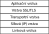
\includegraphics[width=0.3\textwidth]{fig/vrstvy-ssl}
    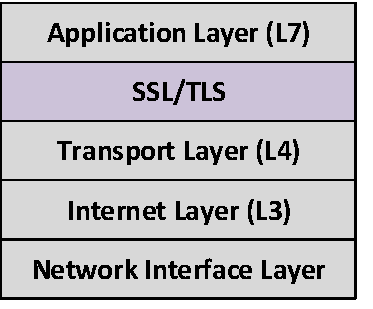
\includegraphics[width=0.3\textwidth]{fig/tls.pdf}
  \caption{Rozšíření modelu TCP/IP o vrstvu SSL/TLS.}
 \label{fig:tls}
\end{figure}

Původní proprietární protokol SSL (navržený firmou Netscape Corporation) byl postupně nahrazen protokolem TLS \cite{RFC7568}. Aktuální doporučená verze protokolu TLS je 1.3~\cite{RFC8446}\footnote{Neformální popis popis standardu TLS je na \url{https://www.davidwong.fr/tls13/}.}.

TLS pracuje na principu klient -- server a vytváří obousměrný zabezpečený kanál pro komunikaci na aplikační vrstvě mezi klientem a serverem. TLS  zajišťuje následující typy zabezpečení:
\begin{itemize}
  \item {\em Autentizace} -- vždy ověřuje identitu serveru (tzv. jednostranná autentizace), která slouží k ochraně komunikace proti útokům typu MITM (Man In the Middle). Může implementovat i oboustrannou autentizaci, kdy klient poskytuje své autentizační údaje server. V praxi se tento přístup příliš nevyužívá. Pro ověřování identity se využívají veřejné klíče a certifikáty X.509, které jsou podepsány certifikační autoritou. 
  \item {\em Důvěrnost (utajení)} -- po navázání spojení a výměně konfiguračních parametrů je obsah přenášené komunikace šifrován. 
  \item {\em Integrita dat} -- TLS zajišťuje ochranu proti modifikaci, vložení či odebrání dat z přenášené komunikace pomocí tzv. kryptografického heše (např. MD4, SHA). 
\end{itemize}

Samotný protokol TLS se skládá ze dvou dílčích protokolů, které jsou součástí zprávy TLS:
\begin{itemize}
  \item \emph{Handshake protocol} se používá při navazování spojení a zajišťuje autentizaci komunikujících stran, výběr kryptografických algoritmů, výměnu parametrů a sdílených klíčů.
  \item \emph{Record protocol} zajišťuje bezpečný přenos mezi komunikujícími stranami.
\end{itemize}

\subsection{Certifikační autority}
Certifikační autorita (CA) je v asymetrické kryptografii subjekt, který vydává digitální (elektronické) certifikáty a ověřuje jejich pravost. Certifikát je elektronický dokument (popsaný v notaci X.500)  potvrzující příslušnost veřejného klíče k dané entitě (službě, serveru, osobě). Certifikační autorita na základě požadavku vygeneruje pro danou entitu dvojici veřejný a soukromý klíč a veřejný klíč s identifikací žadatele vloží do dokumentu zvaného certifikát. Struktura certifikátu je definována standardem X.509 a obsahuje následující informace \cite{rfc5280}:
\begin{itemize}
  \item jméno žadatele (subject)
  \item veřejný klíč žadatele (subject public key)
  \item informace o certifikátu (verze, sériové číslo, doba platnosti)
  \item informace o vydavateli (issuer)
  \item podpis certifikátu (certificate signature), algoritmus a parametry podpisu
\end{itemize}

Pro validaci certifikátu se využívá podpisu certifikační autority, která pomocí svého soukromého klíče podepíše vydaný certifikát. Ověření probíhá pomocí veřejného klíče CA. Jak můžeme ale veřejnému klíči CA důvěřovat? Tento klíč opět musí být podepsán, tzn. musí existovat certifikát, který ověřuje pravost veřejného klíče dané CA. Toto ověření provádí CA vyšší úrovně a vytváří se struktura důvěryhodnosti veřejných klíčů PKI (Public Key Infrastructure). 

Pro ověřování certifikátů nejvyšší úrovně se používají národní a nadnárodní certifikační autority, jejichž veřejné klíče jsou obvykle umístěny přímo ve webových prohlížečích a dalších programech, čímž usnadní uživatelům ověřování důvěryhodnosti webových certifikátů či jiných elektronicky podepsaných dokumentů. 

\subsection{Transparentnost certifikátů}
Aby bylo možné ověřit, že CA vydávají certifikáty poctivě, byl experimentálně zaveden mechanismus transparentnosti certifikátů. Zapojené CA veřejně ohlašují každý vystavený certifikát (případně pre-certifikát). Vydané certifikáty se shromažďují v logovacím souboru {\tt certificate transparency log}, kde může kdokoliv monitorovat nově
přidávané certifikáty a auditovat přítomnost certifikátu nalezených při prohlížení webu.
